% !TEX root = Ausarbeitung.tex

\section{Initial data exploration}
\subsection{Quote\_Id}
\subsubsection{Attribute type: nominal}
The "Quote\_Id" is a customer number. It is neither orderable nor is the number a quantitative value.
\subsubsection{Statistics: } As the attribute is nominal you can not perform any mathematical calculations. The Id ranges between 638 to 434297.

\subsection{Quote\_Date}
\subsubsection{Attribute type: scale}
"Quote\_Date" seems to be at date. These have a specified point of zero. Therefore the type of the attribute is scale.
\subsubsection{Statistics: } 
\textbf{Missing Values}: None

\textbf{Range}: $02/01/2013 - 18/05/2015$


\subsection{Quote\_Flag}
\subsubsection{Attribute type: nominal (dichotomous)}
The description of the attributes declares "Quote\_Flag" as information about whether an insurance was purchased. This can be only answered with yes or no.
\subsubsection{Statistics: }
\textbf{Missing Values}: None

\begin{table}[H]
	\renewcommand{\arraystretch}{1.25}
		\begin{tabular}{l|l|l}
			\textbf{Value} & \textbf{Absolute Frequency} & \textbf{Relative Frequency}\\\hline
			0 & $1605$ & $0.8025$\\ \hline
			1 & $395$ & $0.1975$\\
		\end{tabular}
\end{table}


\subsection{Field\_Info1}
\subsubsection{Attribute type: nominal}
\subsubsection{Statistics: }
\textbf{Missing Values}: None

\begin{table}[H]
	\renewcommand{\arraystretch}{1.25}
	\begin{tabular}{l|l|l}
		\textbf{Value} & \textbf{Absolute Frequency} & \textbf{Relative Frequency}\\\hline
J&$390$ & $0.365\%$\\\hline
F&$540$ & $0.27\%$\\\hline
B&$730$ & $0.195\%$\\\hline
E&$200$ & $0.1\%$\\\hline
C&$39$ & $0.0505\,\%$\\\hline
K&$101$ & $0.0195\%$\\
	\end{tabular}
\end{table}


\subsection{Field\_Info2}
\subsubsection{Attribute type: scale}
All values of "Field\_Info2" are numbers between $0$ and $2$ and have a precision of 4 decimals. This suggests that the values are on a zero-based scale.
\subsubsection{Statistics: }
\begin{table}[H]
	\renewcommand{\arraystretch}{1.25}
	\begin{tabular}{l|l}
		\textbf{Statistic} & \textbf{Value}\\\hline
Missing Values& None\\\hline
Minimum& $0.8746$\\\hline
Maximum& $1.0101$\\\hline
Mean& $0.9391$\\\hline
Std. Dev.& $0.0373$
	\end{tabular}
\end{table}

\paragraph{Histrogramm}:

\subsection{Field\_Info3}
\subsubsection{Attribute type: interval}
\subsubsection{Statistics: }
\paragraph{Missing Values}: None

\subsection{Field\_Info4}
\subsubsection{Attribute type: nominal (dichotomous)}
\subsubsection{Statistics: }
\paragraph{Missing Values}: None

\subsection{Coverage\_Info1}
\subsubsection{Attribute type: interval}
\subsubsection{Statistics: }
\paragraph{Missing Values}: None

\subsection{Coverage\_Info2}
\subsubsection{Attribute type: interval}
\subsubsection{Statistics: }
\paragraph{Missing Values}: None

\subsection{Coverage\_Info3}
\subsubsection{Attribute type: nominal}
\subsubsection{Statistics: }
\paragraph{Missing Values}: None
E	673	0.3365
D	388	0.194
G	245	0.1225
K	229	0.1145
F	221	0.1105
A	116	0.058
J	110	0.055
I	7	0.0035
B	4	0.002
C	3	0.0015
H	2	0.001
L	2	0.001

\subsection{Sales\_Info1}
\subsubsection{Attribute type: nominal (dichotomous)}
\subsubsection{Statistics: }
\paragraph{Missing Values}: None
1	1490	0.745
0	510	0.255

\subsection{Sales\_Info2}
\subsubsection{Attribute type: ordinal}
\subsubsection{Statistics: }
\paragraph{Missing Values}: None
5	1093	0.5465
3	519	0.2595
4	295	0.1475
2	93	0.0465

\subsection{Sales\_Info3}
\subsubsection{Attribute type: nominal}
\subsubsection{Statistics: }
\paragraph{Missing Values}: None

\subsection{Sales\_Info4}
\subsubsection{Attribute type: nominal}
\subsubsection{Statistics: }
\paragraph{Missing Values}: None
K	410	0.205
P	376	0.188
T	332	0.166
Q	312	0.156
V	298	0.149
R	156	0.078
M	116	0.058

\subsection{Sales\_Info5}
\subsubsection{Attribute type: interval}
\subsubsection{Statistics: }
\paragraph{Missing Values}: None

\subsection{Personal\_Info1}
\subsubsection{Attribute type: nominal (dichotomous)}
\subsubsection{Statistics: }
\paragraph{Missing Values}: None
N	1993	0.9965
Y	7	0.0035

\subsection{Personal\_Info2}
\subsubsection{Attribute type: interval}
\subsubsection{Statistics: }
\paragraph{Missing Values}: None

\subsection{Personal\_Info3}
\subsubsection{Attribute type: nominal}
\subsubsection{Statistics: }
\paragraph{Missing Values}: None
ZA	937	0.4685
XR	104	0.052
XM	81	0.0405
XJ	73	0.0365
XD	63	0.0315
XX	62	0.031
XB	59	0.0295
YH	58	0.029
XH	54	0.027
ZT	51	0.0255
XO	50	0.025
ZF	46	0.023
ZR	40	0.02
ZN	39	0.0195
ZH	37	0.0185
XS	35	0.0175
YF	29	0.0145
XW	23	0.0115
ZG	20	0.01
XE	20	0.01
ZW	18	0.009
YE	17	0.0085
ZC	16	0.008
XC	14	0.007
XQ	14	0.007
XL	7	0.0035
ZE	7	0.0035
ZJ	6	0.003
XI	5	0.0025
ZD	5	0.0025
ZK	4	0.002
XZ	4	0.002
ZU	2	0.001

\subsection{Personal\_Info4}
\subsubsection{Attribute type: nominal (dichotomous)}
\subsubsection{Statistics: }
\paragraph{Missing Values}: None
0	1999	0.9995
1	1	0.001
\subsection{Personal\_Info5}
\subsubsection{Attribute type: nominal (dichotomous)}
\subsubsection{Statistics: }
\paragraph{Missing Values}: $966$

\subsection{Property\_Info1}
\subsubsection{Attribute type: nominal (dichotomous)}
\subsubsection{Statistics: }
\paragraph{Missing Values}: $1$
N	1738	0.869
Y	261	0.1305

\subsection{Property\_Info2}
\subsubsection{Attribute type: nominal}
\subsubsection{Statistics: }
\paragraph{Missing Values}: None

\subsection{Property\_Info3}
\subsubsection{Attribute type: nominal}
\subsubsection{Statistics: }
\paragraph{Missing Values}: None
O	573	0.2865
R	533	0.2665
J	285	0.1425
D	198	0.099
S	146	0.073
N	92	0.046
I	77	0.0385
A	31	0.0155
Q	30	0.015
E	10	0.005
H	9	0.0045
K	6	0.003
F	5	0.0025
L	3	0.0015
G	2	0.001

\subsection{Property\_Info4}
\subsubsection{Attribute type: nominal (dichotomous)}
\subsubsection{Statistics: }
\paragraph{Missing Values}: None
1	1364	0.682
0	636	0.318

\subsection{Property\_Info5}
\subsubsection{Attribute type: interval}
\subsubsection{Statistics: }
\paragraph{Missing Values}: None

\subsection{Geographic\_Info1}
\subsubsection{Attribute type: interval}
\subsubsection{Statistics: }
\paragraph{Missing Values}: None

\subsection{Geographic\_Info2}
\subsubsection{Attribute type: interval}
\subsubsection{Statistics: }
\paragraph{Missing Values}: None

\subsection{Geographic\_Info3}
\subsubsection{Attribute type: nominal (dichotomous)}
\subsubsection{Statistics: }
\paragraph{Missing Values}: None
-1	1942	0.971
25	58	0.029

\subsection{Geographic\_Info4}
\subsubsection{Attribute type: nominal (dichotomous)}
\subsubsection{Statistics: }
\paragraph{Missing Values}: None
N	1961	0.9805
Y	39	0.0195

\subsection{Geographic\_Info5}
\subsubsection{Attribute type: nominal}
\subsubsection{Statistics: }
\paragraph{Missing Values}: None
CA	730	0.365
NJ	540	0.27
TX	491	0.2455
IL	239	0.1195

\section{Data Preprocessing}

\section{Summary}


\section{Projektinhalt}
\subsection{Aktivitäten}
\begin{table}[H]
    \renewcommand{\arraystretch}{1.05}
    \begin{center}
        \begin{tabular}{l|l}
            \hline
            \textbf{ID} & \textbf{Aktivität}\\\hline
            A    & Projektmanager\\ \hline
        \end{tabular}
        \caption{Aktivitäten im Projekt}
    \end{center}
\end{table}

\begin{figure}[H]
    \begin{center}
        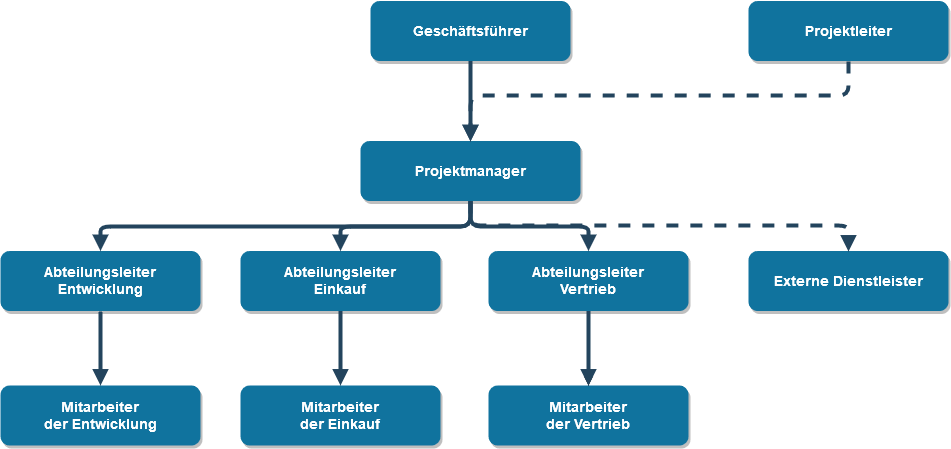
\includegraphics[width=0.8\textwidth]{OBS.png}
    \end{center}
    \caption{Organisation-Breakdown-Strukture}
\end{figure}






